%%%%%%%%%%%%%%%%%%%%%%%%%%%%%%%%%%%%%%%%%%%%%%%%%%%%%%%%%%%%%%%%%%%%%%%%%%%%%%%%%%%%%%%%
%%%%%%%%%%%%%%%%%%%%%%%%%%%%%%%%%%%%%%%%%%%%%%%%%%%%%%%%%%%%%%%%%%%%%%%%%%%%%%%%%%%%%%%%
%%_______ .___________.    ___      .______    _______                      ___       %%
%%|   ____||           |   /   \     |   _  \  |   ____|                   |___ \     %%
%%|  |__   `---|  |----`  /  ^  \    |  |_)  | |  |__          ______        __) |    %%
%%|   __|      |  |      /  /_\  \   |   ___/  |   __|        |______|      |__ <     %%
%%|  |____     |  |     /  _____  \  |  |      |  |____                     ___) |    %%
%%|_______|    |__|    /__/     \__\ | _|      |_______|                   |____/     %%
%%%%%%%%%%%%%%%%%%%%%%%%%%%%%%%%%%%%%%%%%%%%%%%%%%%%%%%%%%%%%%%%%%%%%%%%%%%%%%%%%%%%%%%%
%%%%%%%%%%%%%%%%%%%%%%%%%%%%%%%%%%%%%%%%%%%%%%%%%%%%%%%%%%%%%%%%%%%%%%%%%%%%%%%%%%%%%%%%


%%%%%%%%%%%%%%%%%%%%%%%%%%%%%%%%%%%%%%%%%%%%%%%%%%%%%%%%%%%%%%%%%%%
\section{Étape 3: Extraction de kernels et modélisation de leur performance} \label{sec:methodo_step3}
%%%%%%%%%%%%%%%%%%%%%%%%%%%%%%%%%%%%%%%%%%%%%%%%%%%%%%%%%%%%%%%%%%%


%%%%%%%%%%%%%%%%%
\subsection{Motivations et objectifs}
%%%%%%%%%%%%%%%%%



Les applications que nous ciblons dans notre analyse sont des codes dont la majorité du temps d'exécution se déroule seulement dans quelques pourcentages des lignes de codes. Nous appelons ces zones des points chauds, \textit{hot spots} ou encore \textit{kernels}. Une application possédant des hot spots est un gage d'un potentiel d'amélioration des performances. Les applications réelles utilisées en production dépassent souvent les dizaines de milliers de lignes de codes. Porter et optimiser la totalité d'une application serait complexe et contre-productif. De plus, le portage et l'optimisation des codes est une tâche difficile, même aujourd'hui alors que le nombre d'accélérateurs différents disponibles est réduit. Ensuite, pour optimiser la phase de transformation du code, nous modélisons la performances de ces kernels pour éliminer les plate-formes inadaptées. Ce nombre peut encore être réduite grâce au caractéristiques récupérées lors de l'étape 2.  


L'objectif de cette étape est d'identifier ces zones du code clés et de modéliser leur performances en fonction des performances de la bande passante mémoire (GB/s) ou du processeur (FLOP/s) en calculant leur intensité opérationnelle $\text{OI}_{kernel}$. La majorité des codes étant limité par la performance de la mémoire, la thèse présente un modèle de performance basé sur ses performances. 


%%%%%%%%%%%%%%%%%
\subsection{Identification des kernels}
%%%%%%%%%%%%%%%%%

Si une application passe 99\% de ses cycles dans l'exécution d'une fonction, une amélioration d'un facteur 10 de celle-ci entraînera une amélioration du même facteur de l'application. L'identification des ces fonctions est donc primordiale. 

De nombreux travaux sont réalisés pour identifier et extraire les \textit{hot spots} d'une application \cite{castro2015cere, brunst2013custom}. L'outil de profilage \textit{perf} \cite{de2010new} permet d'extraire un sommaire de l'exécution d'une application en représentant son arbre d'appel (voir \autoref{perf_example}). 



\begin{lstlisting}[caption=Exemple d'utilisation de l'out perf avec la commande \textit{perf record  -g  -F 97}. Le rapport d'exécution est obtenu avec la commande \textit{perf report --stdio}, float,floatplacement=H, label={perf_example}]
# Samples: 116K of event 'cycles:ppp'
# Event count (approx.): 2744862582690
#
# Children      Self  Command          Shared Object       Symbol                                                                       
# ........  ........  ...............  .................. .......
    99.52%     0.00%  Stream.SKL.128   [unknown]           [k] 0000000000000000
            |          
             --99.52%--0
                       |          
                        --99.16%--0xadf96
                                  |
                                  |--25.35%--tuned_STREAM_Add   
                                  |--25.34%--tuned_STREAM_Triad
                                  |--20.36%--tuned_STREAM_Copy
                                  |--17.27%--tuned_STREAM_Scale
                                   --10.74%--main

\end{lstlisting}



%%%%%%%%%%%%%%%%%
\subsection{Modélisation de l'équilibre des kernels}
%%%%%%%%%%%%%%%%%

Chaque kernel peut être porté sur un accélérateur différent, et leur analyse doit se faire indépendamment les uns des autres. L'objectif de la modélisation est de comprendre les performances de l'application: si elles limitées par les performances du sous système mémoire ou par la capacité de calcul du processeur. La modélisation des performances permet de réduire le nombre de plate-forme envisagées pour le portage de l'application. Cette étape permet d'éviter d'investir du temps et de l'argent dans des solutions inefficace pour l'application étudiée. La modélisation du kernel nécessite de lire son code pour compter les différents accès mémoire et les opérations réalisées.

La majorité des codes HPC exécutées sur des architectures modernes voient leurs performances limitées par celle de la bande passante mémoire. S'il est très rare de voir un code limité par la puissance de calcul, il peut être nécessaire de faire cette vérification. 

Pour cela, le \textit{Roof Line Model}, permet de réaliser cette représentation des performances. Il est présenté dans la section \ref{sec:roofline}. 

Il est nécessaire de calculer l'intensité opérationnelle, $\text{OI}_{kernel}$, mesurée en $flop/byte$. Elle représente le nombre d'opération réalisable par le processeur pour chaque donnée transférée depuis la mémoire. Ce calcul se fait à partir de la lecture de code source, motivant le désire des programmeurs d'identifier individuellement les kernels de calculs. 


%%%%%%%%%%%%%%%%%
\subsection{Simple Memory Model: Modélisation de la performance mémoire} \label{sec:smm}
%%%%%%%%%%%%%%%%%

La majorité des codes étant limité par la performance du système mémoire, nous avons développé un modèle de performance simple, permettant de modéliser et valider les performances d'un code facilement. Pour réaliser cette modélisation le développeur doit avoir accès au code source de l'application à porter. Pour un hot spot donné, il faut compter le nombre d'accès mémoire en distinguant les accès en lecture et ceux en écriture. Il est important de distinguer les accès en lecture et en écriture car nous utiliserons leur ratio pour valider le bon comportement de la micro-architecture avec l'outil YAMB. En effet, nous montrons dans notre expérience que la saturation du bus mémoire n'est pas un indicateur suffisant pour conclure de l'efficacité ou non d'un code.

Cette modélisation est faisable seulement si les kernels du code ont été identifiés, l'appliquer sur la totalité de l'application serait trop long. Si la taille des jeux de données $\text{DATA}_{size}$ est connue, il est alors possible de calculer la quantité de donnée minimale qui doit être transférée sur le bus mémoire. Grâce à l'étape 2, nous connaissons les performances maximales théorique $\text{MEMORY}_{peak}$ et réelle $\text{MEMORY}_{max}$ de la micro-architecture. Il est donc possible de calculer la durée optimale pour exécuter fonction étudiée, $\text{TEMPS}_{optimal}$, mesurée en seconde. Le modèle assume que le code utilise un algorithme parfait (utilisation de la localité des données), que sa compilation du code à été réalisée avec un compilateur parfait et qu'il est exécuté sur une plate-forme parfaite. L'objectif n'est pas d'atteindre exactement cette performance, mais de s'en approcher le plus possible. Généralement, lorsque qu'un défaut apparaît à un des niveaux énuméré précédemment, la performance s'éloigne radicalement de la performance optimale.

\begin{equation}
    \text{TEMPS}_{optimal}\ = \frac{\text{DATA}_{size}}{\text{MEMORY}_{max}}
\end{equation}





%%%%%%%%%%%%%%%%%
\subsection{Application des modèles roofline et SMM au benchmark Stream}
%%%%%%%%%%%%%%%%%

L'\autoref{perf_example} montre le profil de l'exécution du benchmark \textit{Stream}. Il comporte quatre fonctions utilisées pour stresser la mémoire par différent type d'accès. Nous choisissons arbitrairement de consacrer notre analyse sur un des quatre \textit{hot spot} de Stream: la fonction \textit{triad} dont le code peut être vu dans l'\autoref{code:triad}. Cette fonction est intéressante car ce motif d'accès est très courant dans les applications HPC (algorithmes RTM).

\subsubsection{Modèle du roofline}
%%%%%%%%%%%%%%%%%
La première étape est de modéliser l'équilibre entre processeur et mémoire des besoins de l'application. 

\begin{lstlisting}[language=c,caption= La fonction triad du benchmark Stream utilise trois matrices: deux en lecture et une en écriture,label={code:triad}, 
  basicstyle=\footnotesize, frame=tb,
  xleftmargin=.065\textwidth, xrightmargin=.065\textwidth]
for (j=0; j < STREAM_ARRAY_SIZE; j++)
    A[j] = B[j] + scalar * C[j];
\end{lstlisting}


Concernant les données, il faut, à chaque itération, charger 3 éléments en double précision, soit 24 bytes. En effet, or optimisation, une ligne de cache doit être chargée avant d'être écrite, même si aucune des données n'est utilisées en lecture par le processeur. Cette fonction a donc une intensité arithmétique $\text{OI}_{kernel} = \frac{2}{24} = 0.083\ flop/byte$.
Pour comparaison, les processeurs récents ont un ratio proche de $10\ flop/byte$. Cette simple modélisation montre le déséquilibre qu'il y a entre la performance de la mémoire et celle des processeurs. Elle permet de guider le choix de la plate-forme sur laquelle cette fonction devra être portée. La \autoref{pic:roofline_stream} montre l'application du roofline à l'étude de la fonction triadd et au processeur étudié. Cette fonction ayant un faible $\text{OI}_{kernel}$, ses performances théorique mesurée en flop sont elles aussi très faible.

\begin{figure}
    \center
    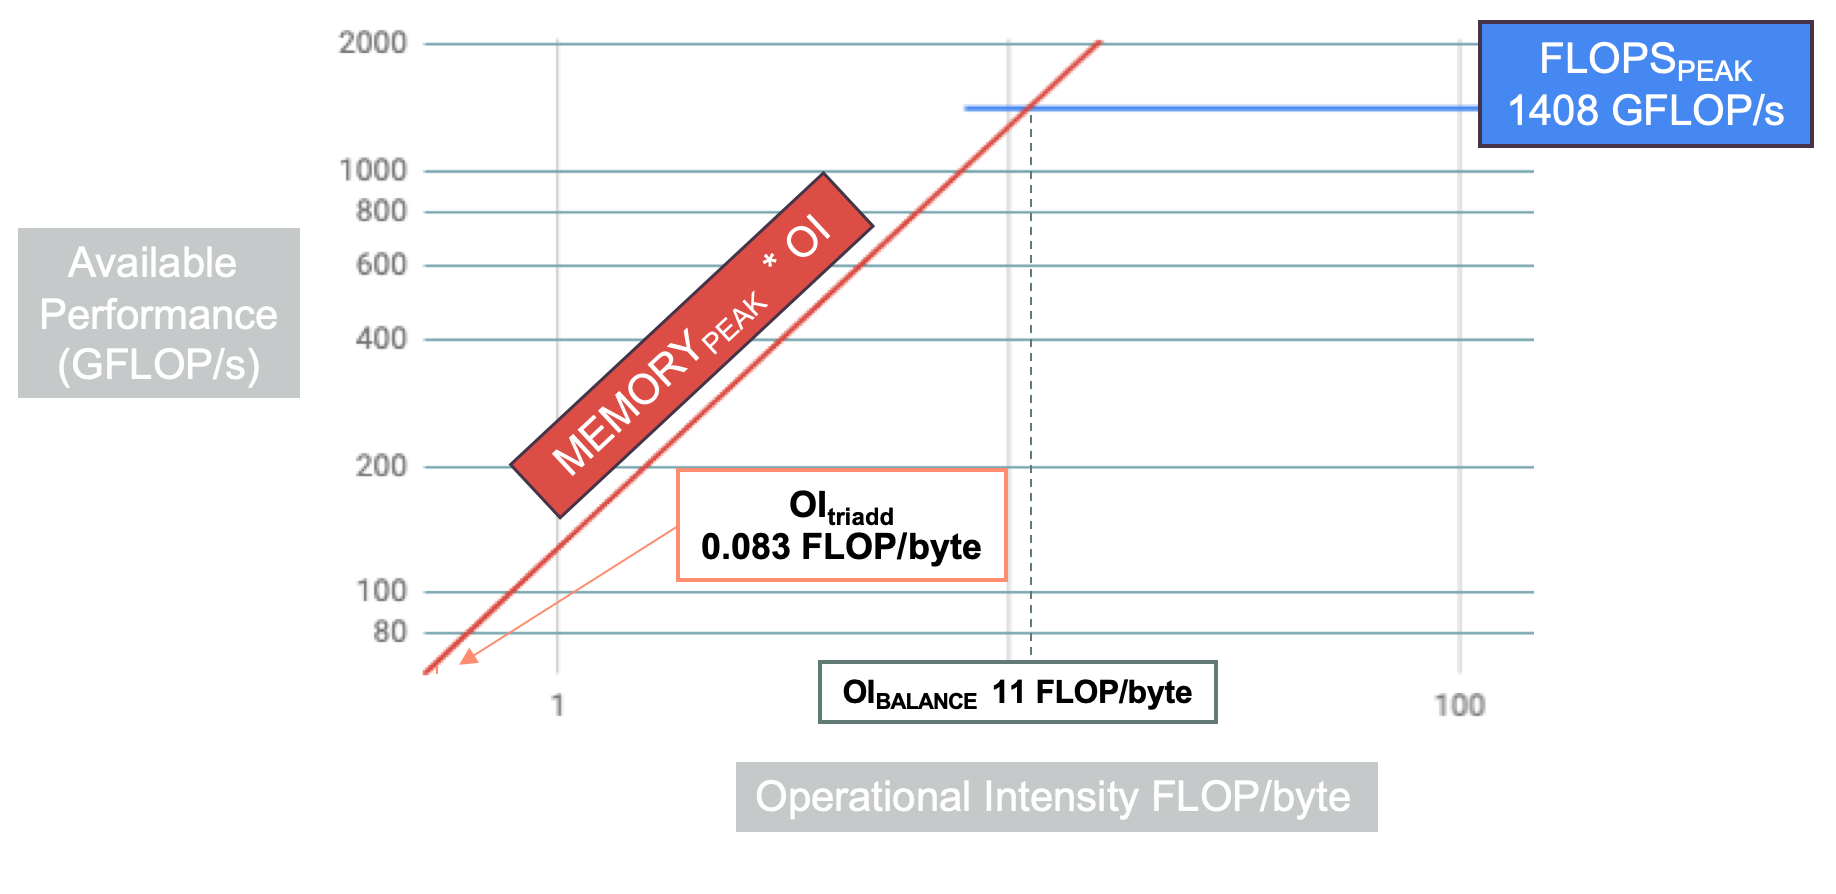
\includegraphics[width=10cm]{images/roofline_stream.png}
    \caption{\label{pic:roofline_stream} Modèle du \textit{Roofline} appliqué à la fonction \textit{triadd} du benchmark \textit{Stream} et un processeur Xeon Skylake 6148.}
\end{figure}



\subsubsection{Simple Memory Model} 
%%%%%%%%%%%%%%%%%
L'analyse de la fonction avec le modèle du \textit{roof line} indique que sur l'architecture ciblée, la performance du code sera limité par la performance de la bande passante.
A chaque itération de boucle, deux opérations doivent être réalisées, une addition et une multiplication. 

Une fois assuré que les performances de l'application sont limitées par le système mémoire, le Simple Memory Model peut être appliqué. Dans notre éxpérimentation, nous utilisons trois matrices de 19.6 GB ($3 \times 10^9 \times sizeof(double)$). Pour une exécution optimale, le bus mémoire devrait être utilisé pour charger une fois les deux matrices en lectures (matrices B et C)  et pour l'écriture de la matrice A. Le traffic mémoire total serait alors de 58.8 GB. En utilisant les résultats mesurés lors de l'étape 2, on peut estimer le temps optimale pour l'exécution de cette fonction: $\text{TEMPS}_{optimal} = \frac{58.8}{128} = 0.56$ seconde.